\chapter{Interfejs użytkownika}
Użytkownik wchodzi w interakcję z systemem poprzez aplikację webową, która jest dostępna w przeglądarce internetowej.
Za jej pomocą może on przeglądać strumienie wideo z kamer oraz zarządzać konfiguracją detekcji.

\section{Architektura modułu}
\subsection{Stos technologiczny}
Aplikacja webowa została zbudowana na podstawie szkieletu aplikacji \texttt{Next.js}. 
W roku 2026 najpopularniejszymi szkieletami aplikacji webowych pozostają \texttt{Vite} oraz właśnie \texttt{Next.js}.
Prawdopodobnie obie technologie sprawdziłyby się w tym projekcie, ale wybór padł na \texttt{Next.js} ze względu na to, że jest technologią nowszą.

Za warstwę wizualną odpowiada biblioteka \texttt{React}, która jest obecnie najpopularniejszą biblioteką do tworzenia interfejsów użytkownika w języku \texttt{JavaScript}. Zamiast klasycznego \texttt{JS} użyto jednak \texttt{TypeScript}, który wprowadza typowanie statyczne do języka \texttt{JavaScript}, co pozwala na wcześniejsze wykrywanie błędów w kodzie.

Warstwa stylistyczna została zrealizowana przy pomocy biblioteki \texttt{TailwindCSS}, która wprowadza gotowe klasy \texttt{CSS}, pozwalające na szybkie tworzenie estetycznych interfejsów użytkownika. Wykorzystano też gotowe komponenty z bilbioteki \texttt{shadcn/ui}, która jest zbiorem komponentów \texttt{React} stworzonych w oparciu o \texttt{TailwindCSS}. Część komponentów wzorowana jest na komponentach ze strony \href{https://flowbite.com}{\texttt{Flowbite}}.

Dodatkowo wykorzystano następujące biblioteki: 
\begin{itemize}
\item \texttt{Orval} --- biblioteka do generowania klienta API na podstawie specyfikacji \texttt{OpenAPI} (dawniej \texttt{Swagger}). Pozwala na automatyczne generowanie kodu, który umożliwia komunikację z serwerem poprzez protokół \texttt{HTTP}.
\item \texttt{Tanstack Query} --- biblioteka do zarządzania stanem aplikacji oraz komunikacją z serwerem. Umożliwia łatwe pobieranie danych z serwera oraz ich buforowanie w pamięci podręcznej, co pozwala na szybsze działanie aplikacji.
\item \texttt{Zustand} --- biblioteka do zarządzania stanem aplikacji. Umożliwia łatwe zarządzanie stanem globalnym w aplikacji \texttt{React}.
\item \texttt{Axios} --- biblioteka do wykonywania zapytań \texttt{HTTP}. Umożliwia łatwe wysyłanie zapytań do serwera oraz obsługę odpowiedzi.
\item \texttt{Shaka-Player} --- biblioteka do odtwarzania strumieni wideo w formacie \texttt{MPEG-DASH}. Umożliwia odtwarzanie strumieni wideo w przeglądarce internetowej.
\item \texttt{Zod} --- biblioteka do walidacji danych. Umożliwia łatwe sprawdzanie poprawności danych wprowadzanych przez użytkownika. 
\end{itemize}

\subsection{Implementacja}
\begin{figure}[H]
    \centering
    \begin{tikzpicture}[
        base/.style={draw, rectangle, rounded corners=3pt, align=center, font=\small, inner sep=5pt},
        external/.style={base, draw=red!60!black, fill=red!5!, thick, dashed, minimum width=5cm, minimum height=0.8cm},
        client/.style={base, draw=blue!60!black, fill=blue!5!, thick, minimum width=5cm, minimum height=0.8cm},
        comp/.style={base, draw=green!60!black, fill=green!5!, minimum width=2.4cm},
        hook/.style={base, draw=purple!70!black, fill=purple!5!, font=\scriptsize, minimum width=1.1cm},
        store/.style={base, draw=orange!70!black, fill=orange!5!, font=\scriptsize, minimum width=1.1cm},
        box/.style={draw=gray!40, fill=gray!5, dashed, rounded corners=5pt, inner sep=10pt},
        boxtitle/.style={font=\small\bfseries, text=gray!80!black},
        arrow/.style={-{Stealth[scale=1.2]}, thick, draw=gray!80!black},
        botharrow/.style={{Stealth[scale=1.2]}-{Stealth[scale=1.2]}, thick, draw=gray!80!black},
        dot/.style={circle, fill=gray!60, inner sep=0pt, minimum size=4pt}
    ]
    % 1. WARSTWA PODSTAWOWA (DÓŁ)
    \node[external] (api) {Zewnętrzny Serwer API\\(np. \texttt{FastAPI})};
    \node[client, above=1.2cm of api] (client) {Klient API (Axios / Fetch)};
    % 2. KOLUMNY FUNKCJONALNOŚCI (ŚRODEK I GÓRA)
    % --- FUNKCJONALNOŚĆ 1 (Lewa) ---
    \node[hook, above left=1.8cm and 1.2cm of client.north] (h1) {Hook};
    \node[store, right=0.2cm of h1] (s1) {Store};
    \node[comp, above=0.6cm of h1.north east] (c1) {Komponent UI};
    % --- FUNKCJONALNOŚĆ 2 (Prawa) ---
    \node[hook, above right=1.8cm and 1.2cm of client.north] (h2) {Hook};
    \node[store, right=0.2cm of h2] (s2) {Store};
    \node[comp, above=0.6cm of h2.north east] (c2) {Komponent UI};
    % 3. GENEROWANIE KONTENERÓW (TŁO)
    \begin{scope}[on background layer]
        \node[box, fit=(h1) (s1) (c1)] (box1) {};
        \node[box, fit=(h2) (s2) (c2)] (box2) {};
    \end{scope}
    % Podpisy pod kontenerami
    \node[boxtitle, above=2pt of box1.north] {Funkcjonalność 1};
    \node[boxtitle, above=2pt of box2.north] {Funkcjonalność 2};
    % --- TRZY KROPKI Z PRAWEJ STRONY ---
    \node[right=1.2cm of box2] (ellipsis) {};
    \node[dot, left=5pt of ellipsis] {};
    \node[dot] at (ellipsis) {};
    \node[dot, right=5pt of ellipsis] {};
    % 4. POŁĄCZENIA (STRZAŁKI)
    \draw[botharrow] (api) -- node[right, font=\tiny, text=gray!60!black] {HTTP / JSON} (client);
    \draw[arrow] (client.north) -- (box1.south);
    \draw[arrow] (client.north) -- (box2.south);
    \draw[arrow] (h1.north) -- (c1.south west);
    \draw[arrow] (s1.north) -- (c1.south east);
    \draw[arrow] (h2.north) -- (c2.south west);
    \draw[arrow] (s2.north) -- (c2.south east);
    \end{tikzpicture}
    \caption{Modularny podział warstwy prezentacyjnej z wyodrębnieniem domen funkcjonalnych.}\label{fig:modular_architecture_diagram}
\end{figure}
Aplikacja jest jednostronna (ang. \textit{Single Page Application}), co oznacza, że nie wykorzystuje ona trasowania po stronie serwera i działa jedynie w korzeniu domeny.

Zastosowana architektura modułu interfejsu użytkownika jest zorientowana na funkcjonalności (ang. \textit{Feature-Driven Architecture}). Oznacza to, że każda funkcjonalność ma własne komponenty interfejsu użytkownika, jak i również magazyny i hooki. Część podmodułów jest wspólna dla całego modułu, np.\ komponenty \texttt{shadcn/ui}. Podobnie jest z klientem API, z którego korzystają wszystkie funkcjonalności. 

Wspomniane hooki i magazyny (ang. \textit{store}) są wykorzystywane do zarządzania stanem aplikacji. Mają one jednak różne zastosowania. Magazyny przechowują te dane, które modyfikowane są przez użytkownika np.\ zaznaczone nagrania do usunięcia. Z kolei hooki są wykorzystywane do pobierania danych z serwera i ich buforowania w pamięci podręcznej. Dodatkowo częściowo realizują też komunikację w drugą stronę, np.\ przekazując nowe szablony detekcji. 

\section{Opis funkcjonalności}

\subsection{Obsługa motywów}
Moduł interfejsu użytkownika obsługuje dwa motywy: jasny i ciemny. Co prawda nie istnieje żaden przełącznik w interfejsie użytkownika, który pozwalałby na zmianę motywu, ale można to uczynić poprzez zmianę ustawień systemowych w przeglądarce internetowej, do której dopasowuje się aplikacja.

\begin{figure}[H]
    \centering
    \begin{subfigure}{0.45\textwidth}
        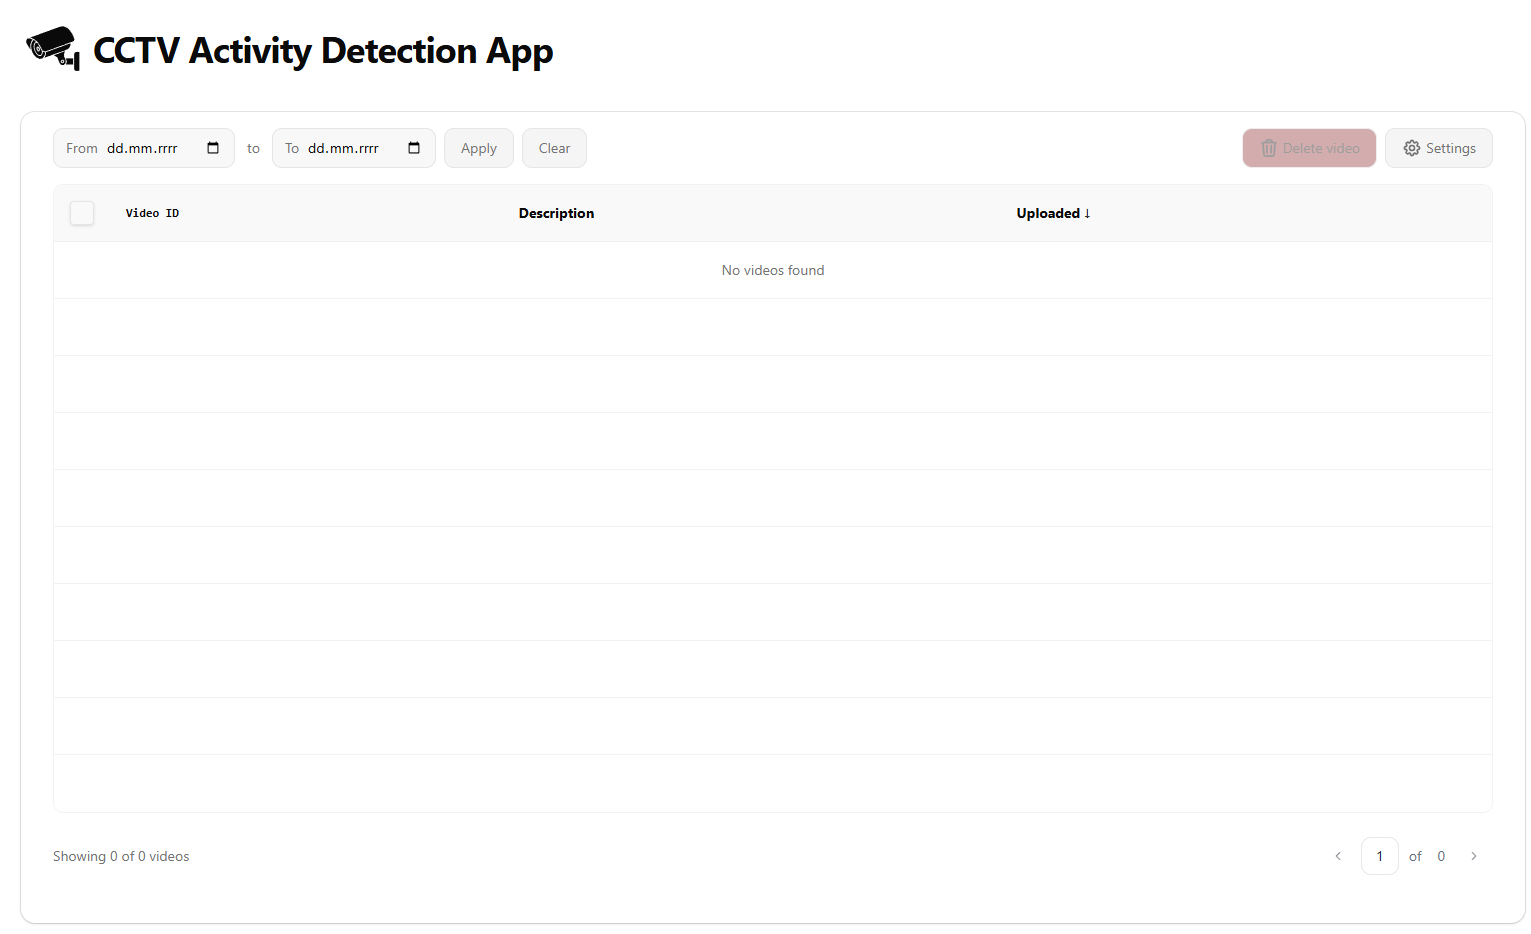
\includegraphics[width=0.95\textwidth]{images/frontend/interfejs_jasny.png}
        \subcaption{Motyw jasny.}\label{fig:frontend_light_theme}
    \end{subfigure}
    \hfill
    \begin{subfigure}{0.45\textwidth}
        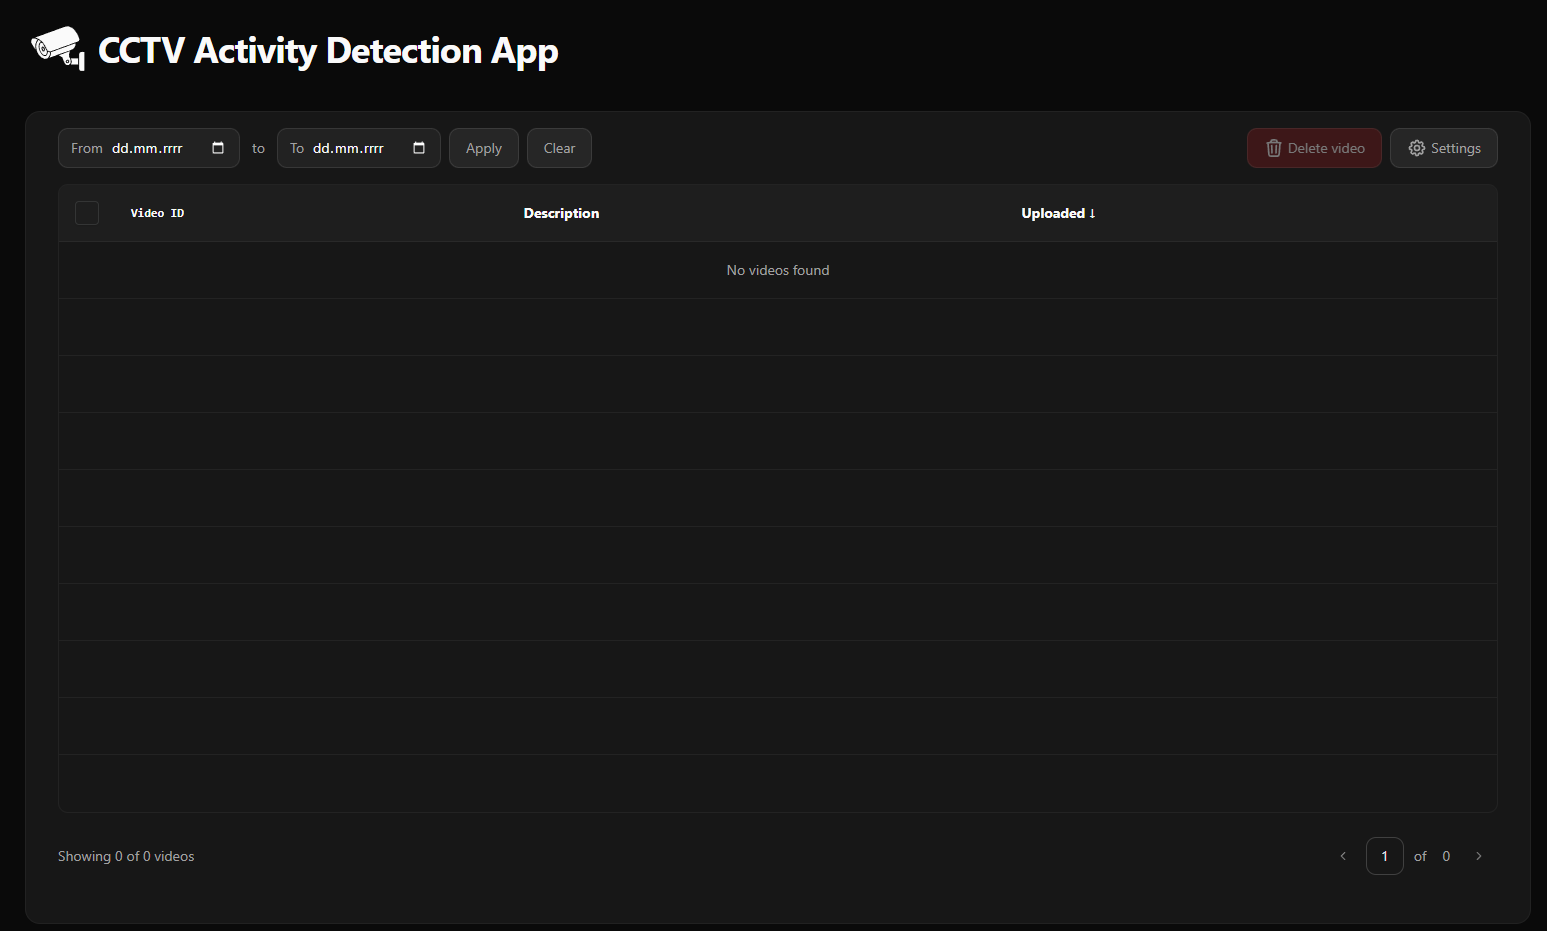
\includegraphics[width=0.95\textwidth]{images/frontend/interfejs_ciemny.png}
        \subcaption{Motyw ciemny.}\label{fig:frontend_dark_theme}
    \end{subfigure}

    \caption{Widok aplikacji w motywach jasnym i ciemnym.}
\end{figure}

\subsection{Lista i wyświetlacz nagrań}

\begin{figure}[H]
    \centering
    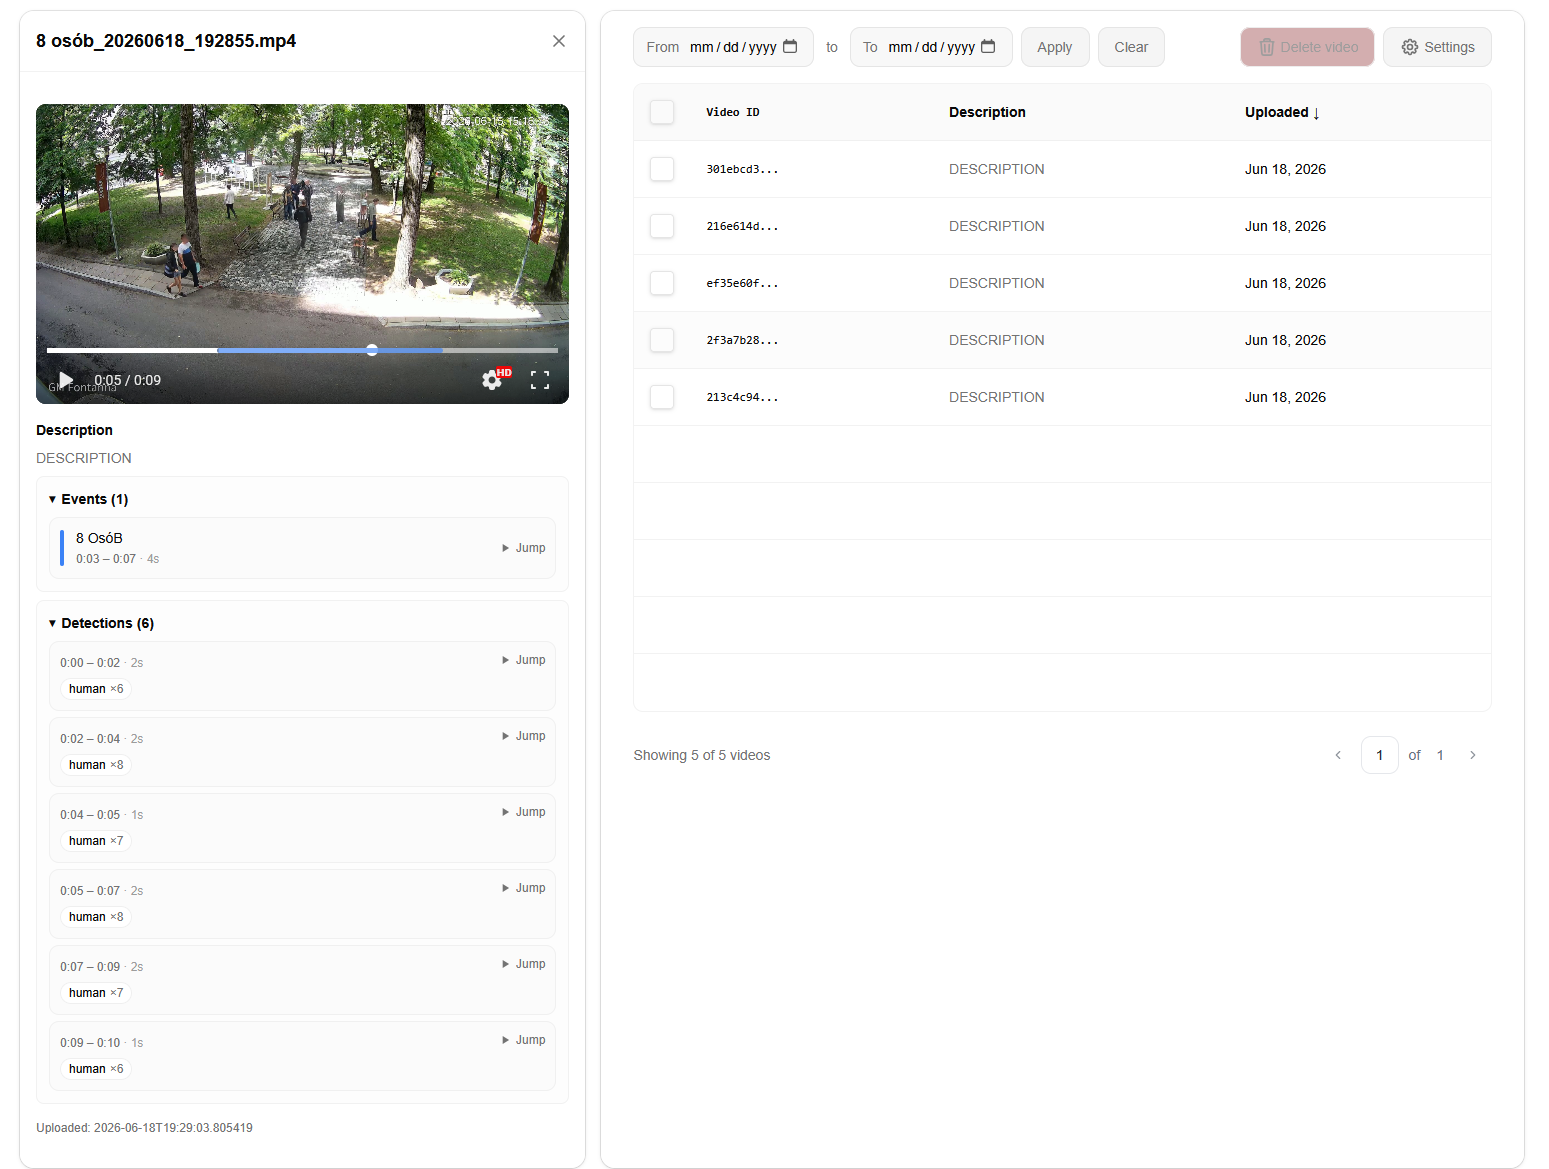
\includegraphics[width=0.95\textwidth]{images/frontend/interfejs.png}
    \caption{Lista nagrań wideo z możliwością ich odtwarzania.}\label{fig:frontend_recordings_list}
\end{figure}

Na \myref[rysunku]{fig:frontend_recordings_list} przedstawiono listę nagrań wideo. Widać, że jest ich pięć (\textit{Showing 5 of 5 videos}) oraz że wszystkie są na jednej stronie (\textit{1 of 1}). Każde nagranie posiada opis (nie zaimplementowano uzyskiwania opisów za pomocą wizyjnego modelu językowego), listę zarejestrowanych zdarzeń oraz zarejestrowanych detekcji z przedziałami czasowymi, w których mają miejsce.
Wyświetlacz nagrań można zmaksymalizować, ale wbrew temu, co może sugerować umieszczona na nim zębatka, niemożliwa jest zmiana jakości przesyłanego strumienia wideo. 

\subsubsection{Filtrowanie po dacie}
\begin{figure}[H]
    \centering
    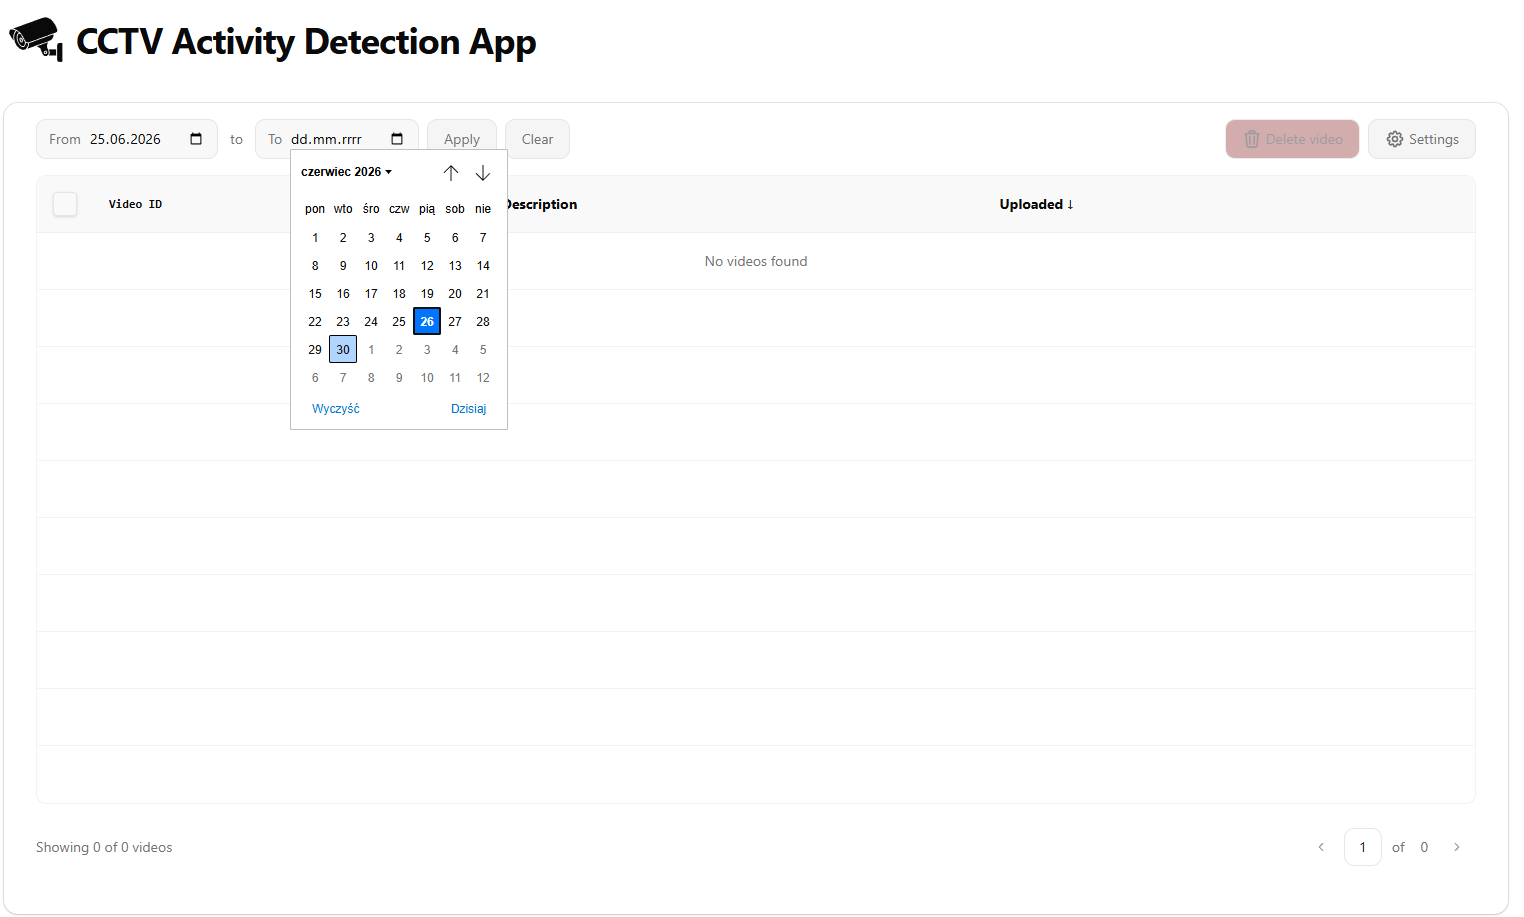
\includegraphics[width=0.95\textwidth]{images/frontend/filtrowanie.png}
    \caption{Filtrowanie nagrań wideo po dacie.}\label{fig:frontend_date_filter}
\end{figure}

Aplikacja umożliwia filtrowanie nagrań wideo po dacie. Na \myref[rysunku]{fig:frontend_date_filter} przedstawiono widok, na którym wybrano już dolny przedział daty od 25 czerwca 2026 r., a górny jest dopiero w trakcie wybierania. Nie wyświetliło się żadne z nagrań.

\subsubsection{Usuwanie nagrań}
\begin{figure}[H]
    \centering
    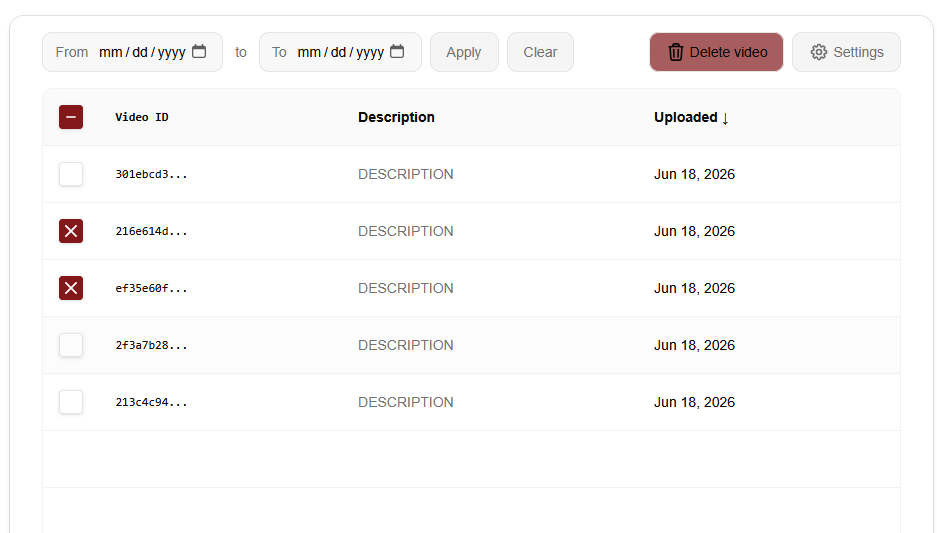
\includegraphics[width=0.95\textwidth]{images/frontend/usuwanie.png}
    \caption{Usuwanie nagrań wideo.}\label{fig:frontend_delete_recordings}
\end{figure}
Powyższy rysunek przedstawia zaznaczone do usunięcia nagrania wideo. Po kliknięciu przycisku \textit{Delete video} na serwer API trafi żądanie usunięcia nagrań z bazy danych.

\subsection{Ustawienia detekcji zdarzeń}

\begin{figure}[H]
    \centering
    \begin{subfigure}{0.49\textwidth}
        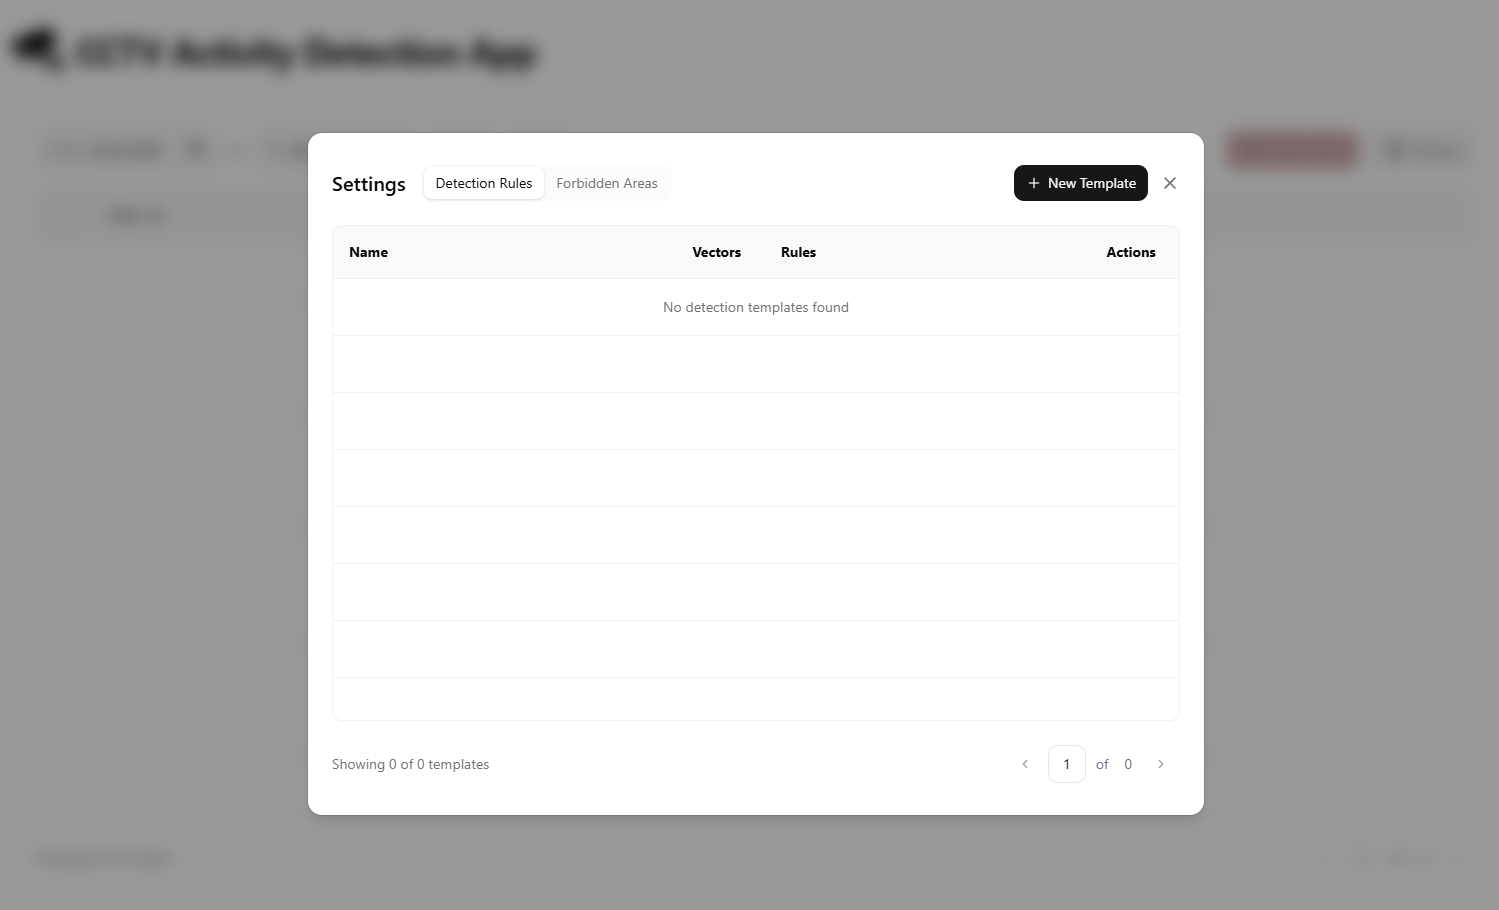
\includegraphics[width=0.95\textwidth]{images/frontend/zasady_wykrywania.png}
        \subcaption{Szablony detekcji.}
    \end{subfigure}
    \hfill
    \begin{subfigure}{0.49\textwidth}
        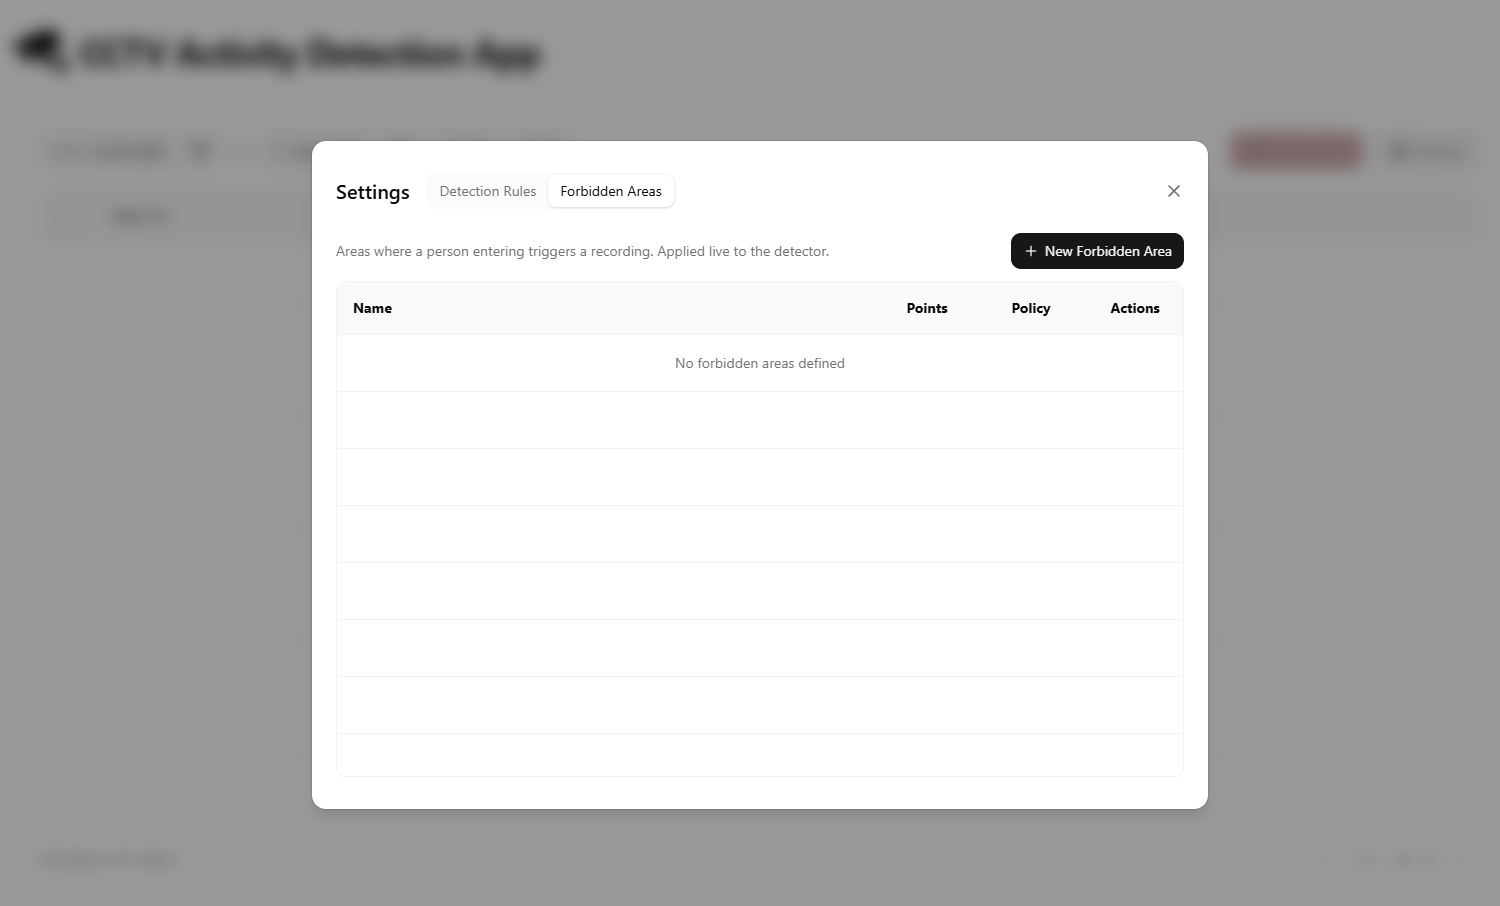
\includegraphics[width=0.95\textwidth]{images/frontend/zakazane_obszary.png}
        \subcaption{Wykrywane obszary.}
    \end{subfigure}
    \caption{Widok ustawień.}\label{fig:frontend_settings}
\end{figure}

Ustawienia dzielą się na dwie sekcje przedstawione na \myref[rysunku]{fig:frontend_settings}. W pierwszej z nich użytkownik może zarządzać szablonami detekcji, a w drugiej wykrywanymi obszarami.
\begin{figure}[H]
    \centering
    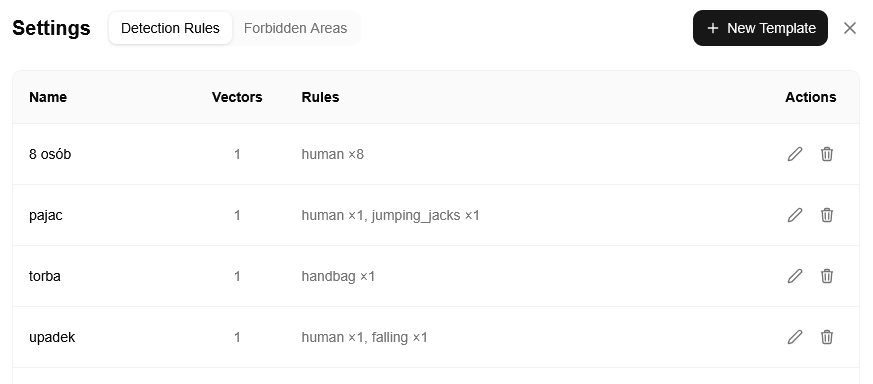
\includegraphics[width=0.95\textwidth]{images/frontend/wektory_wykryc.png}
    \caption{Przykład wprowadzonych szablonów wykryć.}\label{fig:frontend_detection_vectors}
\end{figure}

Jak widać na \myref[rysunku]{fig:frontend_detection_vectors}, użytkownik może zarządzać wprowadzonymi szablonami wykryć poprzez ich edycję, dodawanie i usuwanie.

\begin{figure}[H]
    \centering
    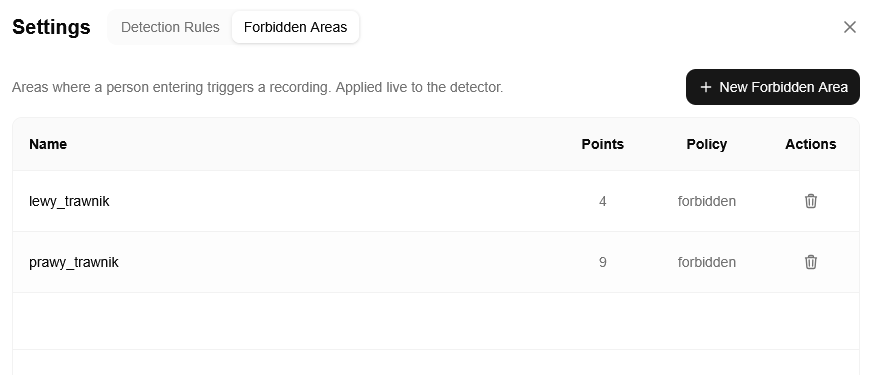
\includegraphics[width=0.95\textwidth]{images/frontend/obszary_wykluczone.png}
    \caption{Przykład wprowadzonych zakazanych obszarów.}\label{fig:frontend_restricted_areas}
\end{figure}

W przypadku zakazanych obszarów niemożliwe jest ich edytowanie, a jedynie dodawanie i usuwanie. Na \myref[rysunku]{fig:frontend_restricted_areas} pokazane są dwa zakazane obszary, które zostały wprowadzone przez użytkownika.

\subsection{Dodawanie szablonów detekcji}
\begin{figure}[H]
    \centering
    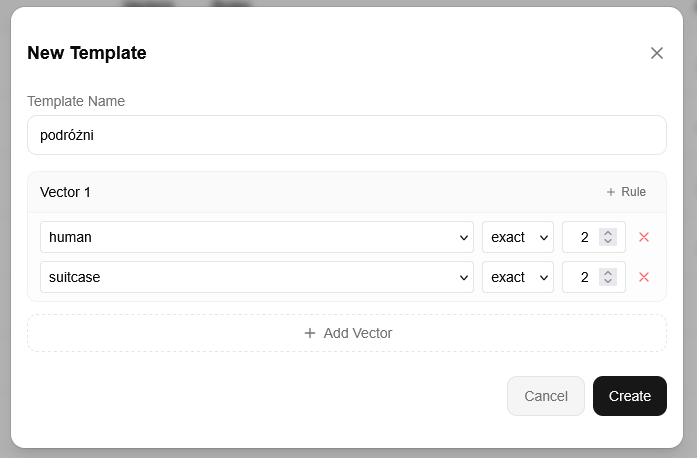
\includegraphics[width=0.95\textwidth]{images/frontend/wektor_podrozni.png}
    \caption{Przykład dodawania szablonu wykryć.}
\end{figure}
Powyższy rysunek przedstawia dodawanie szablonu wykryć. W tym przypadku użytkownik wprowadza szablon złożony z pojedynczego wektora, który wykrywa 2 ludzi i 2 teczki. Samo wprowadzenie szablonu nie wystarcza, aby zapisał się on w bazie danych. Konieczne jest wciśnięcie przycisku \enquote{Create}.

\subsection{Dodawanie zakazanych obszarów}
\begin{figure}[H]
    \centering
    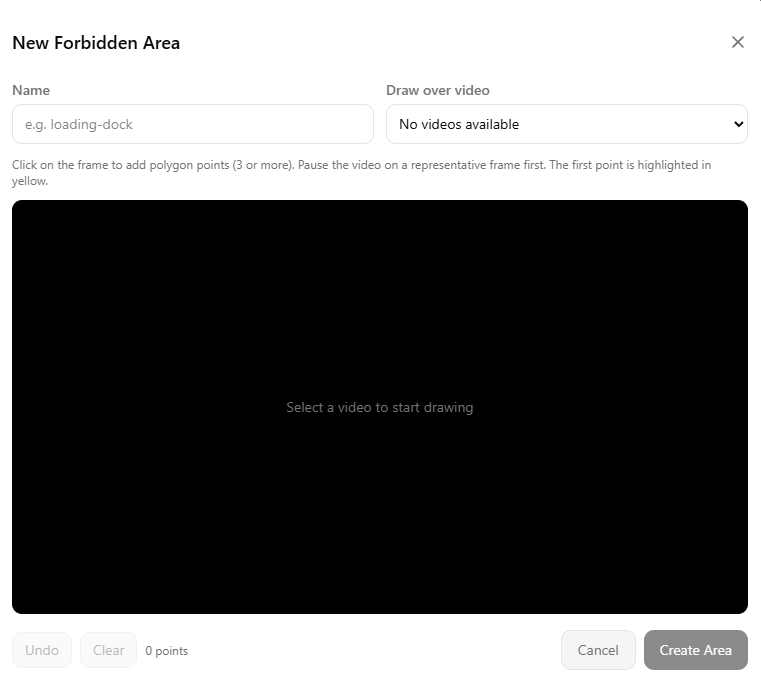
\includegraphics[width=0.95\textwidth]{images/frontend/zakazane_obszary_dodawanie.png}
    \caption{Przykład dodawania zakazanego obszaru.}
\end{figure}
Funkcjonalność pozwala na tworzenie wielokątów na obrazie z kamery, które będą traktowane jako zakazany obszar. Poniżej przykłady obszarów lewego i prawego trawnika:
\begin{figure}[H]
    \centering
    \begin{subfigure}{0.49\textwidth}
        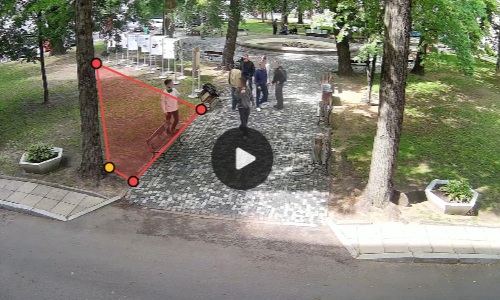
\includegraphics[width=0.95\textwidth]{images/frontend/lewy_trawnik.png}
        \subcaption{Lewy trawnik.}
    \end{subfigure}
    \hfill
    \begin{subfigure}{0.49\textwidth}
        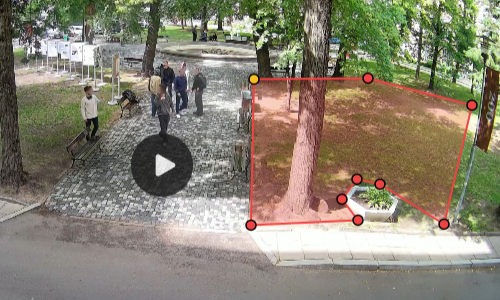
\includegraphics[width=0.95\textwidth]{images/frontend/prawy_trawnik.png}
        \subcaption{Prawy trawnik.}
    \end{subfigure}
    \caption{Zaznaczone obszary.}\label{fig:frontend_grass_areas}
\end{figure}
Wymagane jest zatem, aby w bazie danych były już zarejestrowane jakieś nagrania wideo, aby można było na ich podstawie wyznaczyć zakazane obszary. 